\clearpage
\newpage
\section{Schedule and Milestones}

The schedule is shown in Figure~\ref{fig:sandm} and the milestones are listed in Table~\ref{tab:milestones}.

\begin{table}[ht]
\centering
\caption{The project has the following fourteen (14) milestones}

{\scriptsize
\begin{tabular}{|m{.25in}|m{.25in}|m{4.0in}|m{1.65in}|} 
\hline
Mile-stones & Month & Description & Deliverables \\ \hline
1 & 2 & Initial Design completed.  Design includes finalized research plans, identification of internal TA milestones, initial interfaces between the three TAs, planned interface with the TA4 platforms. &  \\ \hline
2 & 3 & Individual components developed and tested.   TA1, TA2 and TA3 Interface design completed & Quarterly Report \\ \hline
3 & 6 & Initial working system for Design Time (i.e., TA1 – TA3 interaction).  Continued development of TA2.  Supports includes one LEC.   First P/I meeting.   Review TA4 scenarios. & Quarterly Report, slide presentation \\ \hline
4 & 12 & Working system for both Design Time and Operation Time (i.e., TA1, TA2 and TA3 interactions), supports 10 dimensions and one LEC.  Second P/I meeting.   Initial discussions with TA4 teams on interfaces & Quarterly Report, slide presentation \\ \hline
5 & 17 & Working system that supports 20 dimensions and 2 LECs with no more that 50\% monitoring overhead, 10 conditional evidence monitors and 0.1x reduced trails to assurance.   Start integration effort into both TA4 platforms & Working system (software) available for integration into TA4 platforms.  Monthly perfomance and financial reports \\ \hline
6 & 18 & Phase I demonstration on both TA4 platforms & Phase I report, quarterly reports \\ \hline
7 & 19 & Design review based on Phase I demo (lessons learned). &  \\ \hline
8 & 25.5 & Prototype system capable of supporting 30 dimensions, 3 LECs, with no more than 40\% monitoring overhead, 50 conditional evidence and 0.05x reduced trails to assurance.   Third P/I meeting & Quarterly report \\ \hline
9 & 32 & Working system that supports up to 40 dimensions, 4 LECs, with no more than 30\% monitoring overhead, 100 conditional evidence monitors and 0.01x reduced trails to assurance.  Begin Integration into both TA4 platforms & Working system (software) available for integration into TA4 platforms.  Monthly perfomance and financial reports \\ \hline
10 & 33 & Phase II demonstration on both TA4 platforms & Phase II report, quarterly reports \\ \hline
11 & 34 & Design review based on Phase II demo (lessons learned) &  \\ \hline
12 & 40.5 & Refined system to support 70 dimensions, 5 LECs, 500 conditional evidences and 20\% monitoring overhead – Forth P/I meeting & Quarterly report \\ \hline
13 & 47 & Working system that supports 100 dimensions, 6 LECs, 1000 conditional evidences, .001x reduction in assurance trials and 10\% monitoring overhead & Working system (software) available for integration into TA4 platforms.  Monthly perfomance and financial reports \\ \hline
14 & 48 & Phase III demonstration on both TA4 platforms. Phase III report, final project reporet. & Phase III report, quarterly reports, Final project report \\ \hline
\end{tabular}
}
\label{tab:milestones}
\end{table}

\begin{figure}[tbhp]
\begin{center}
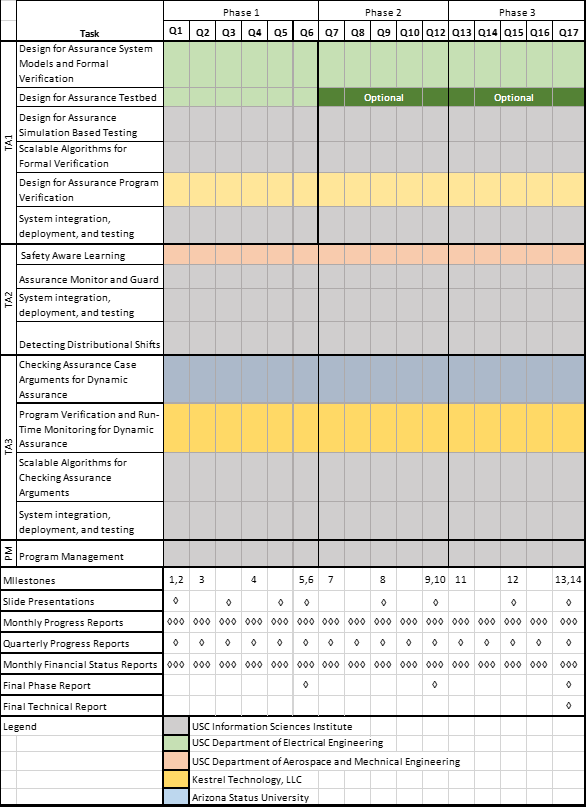
\includegraphics[width=.95\textwidth]{figs/Safeguard_Schedule_V6}
\end{center}
\vspace{-.2in}\caption{Project schedule along with a summary of milestones.  The legend maps task color to organization primary responsible for the task. } 
\label{fig:sandm}
\end{figure}
 